\documentclass[aspectratio=169]{../latex_main/tntbeamer}  % you can pass all options of the beamer class, e.g., 'handout' or 'aspectratio=43'
\usepackage{dsfont}
\usepackage{bm}
\usepackage[english]{babel}
\usepackage[T1]{fontenc}
%\usepackage[utf8]{inputenc}
\usepackage{graphicx}
\graphicspath{ {./figures/} }
\usepackage{algorithm}
\usepackage[ruled,vlined,algo2e,linesnumbered]{algorithm2e}
\usepackage{hyperref}
\usepackage{booktabs}
\usepackage{mathtools}

\usepackage{amsmath,amssymb}

\DeclareMathOperator*{\argmax}{arg\,max}
\DeclareMathOperator*{\argmin}{arg\,min}

\usepackage{pgfplots}
\pgfplotsset{compat=1.16}
\usepackage{tikz}
\usetikzlibrary{trees} 
\usetikzlibrary{shapes.geometric}
\usetikzlibrary{positioning,shapes,shadows,arrows,calc,mindmap}
\usetikzlibrary{positioning,fadings,through}
\usetikzlibrary{decorations.pathreplacing}
\usetikzlibrary{intersections}
\pgfdeclarelayer{background}
\pgfdeclarelayer{foreground}
\pgfsetlayers{background,main,foreground}
\tikzstyle{activity}=[rectangle, draw=black, rounded corners, text centered, text width=8em]
\tikzstyle{data}=[rectangle, draw=black, text centered, text width=8em]
\tikzstyle{myarrow}=[->, thick, draw=black]

% Define the layers to draw the diagram
\pgfdeclarelayer{background}
\pgfdeclarelayer{foreground}
\pgfsetlayers{background,main,foreground}

% Requires XeLaTeX or LuaLaTeX
\usepackage{unicode-math}

\usepackage{fontspec}
%\setsansfont{Arial}
\setsansfont{RotisSansSerifStd}[ 
Path=../latex_main/fonts/,
Extension = .otf,
UprightFont = *-Regular,  % or *-Light
BoldFont = *-ExtraBold,  % or *-Bold
ItalicFont = *-Italic
]
\setmonofont{Cascadia Mono}[
Scale=0.8
]

% scale factor adapted; mathrm font added (Benjamin Spitschan @TNT, 2021-06-01)
%\setmathfont[Scale=1.05]{Libertinus Math}
%\setmathrm[Scale=1.05]{Libertinus Math}

% other available math fonts are (not exhaustive)
% Latin Modern Math
% XITS Math
% Libertinus Math
% Asana Math
% Fira Math
% TeX Gyre Pagella Math
% TeX Gyre Bonum Math
% TeX Gyre Schola Math
% TeX Gyre Termes Math

% Literature References
\newcommand{\lit}[2]{\href{#2}{\footnotesize\color{black!60}[#1]}}

%%% Beamer Customization
%----------------------------------------------------------------------
% (Don't) Show sections in frame header. Options: 'sections', 'sections light', empty
\setbeamertemplate{headline}{empty}

% Add header logo for normal frames
\setheaderimage{
	% 
\includegraphics[height=\logoheight]{figures/TNT_darkv4.pdf}
	
\includegraphics[height=\logoheight]{../latex_main/figures/luh_logo_rgb_0_80_155.pdf}
	% 
\includegraphics[height=\logoheight]{figures/logo_tntluh.pdf}
}

% Header logo for title page
\settitleheaderimage{
	% 
\includegraphics[height=\logoheight]{figures/TNT_darkv4.pdf}
	
\includegraphics[height=\logoheight]{../latex_main/figures/luh_logo_rgb_0_80_155.pdf}
	% 
\includegraphics[height=\logoheight]{figures/logo_tntluh.pdf}
}

% Title page: tntdefault 
\setbeamertemplate{title page}[tntdefault]  % or luhstyle
% Add optional title image here
%\addtitlepageimagedefault{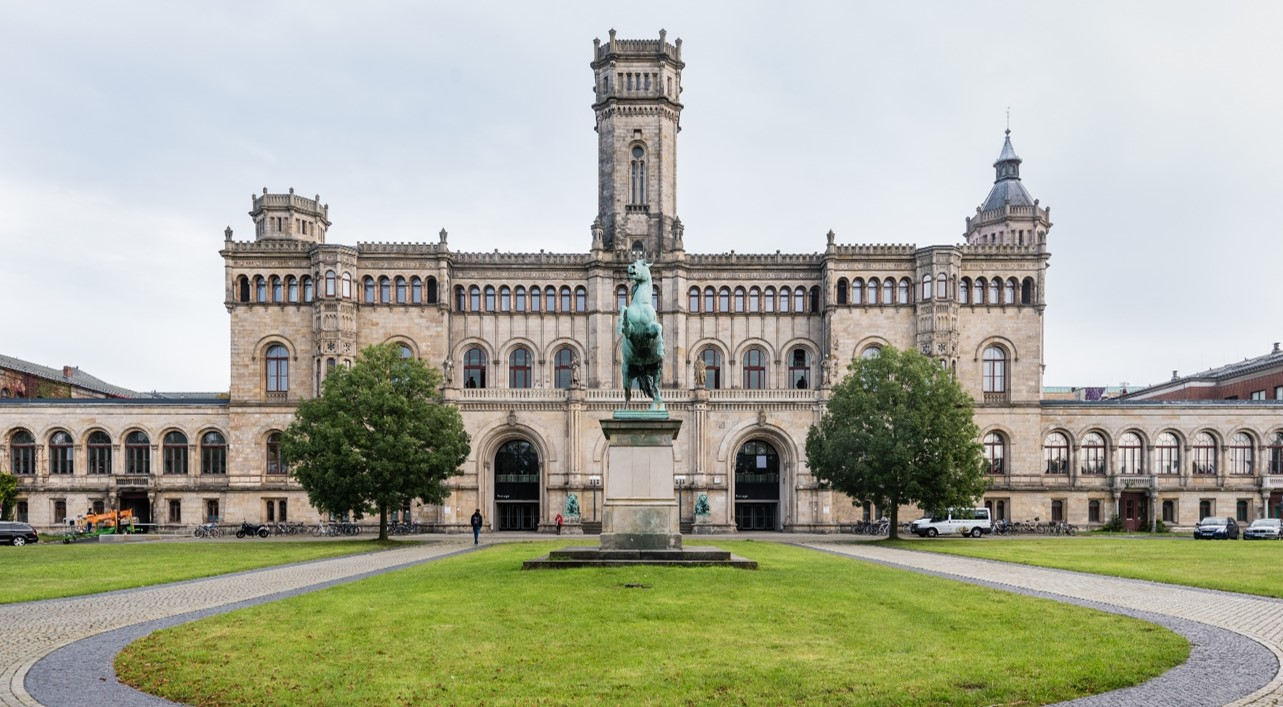
\includegraphics[width=0.65\textwidth]{figures/luh_default_presentation_title_image.jpg}}

% Title page: luhstyle
% \setbeamertemplate{title page}[luhstyle]
% % Add optional title image here
% \addtitlepageimage{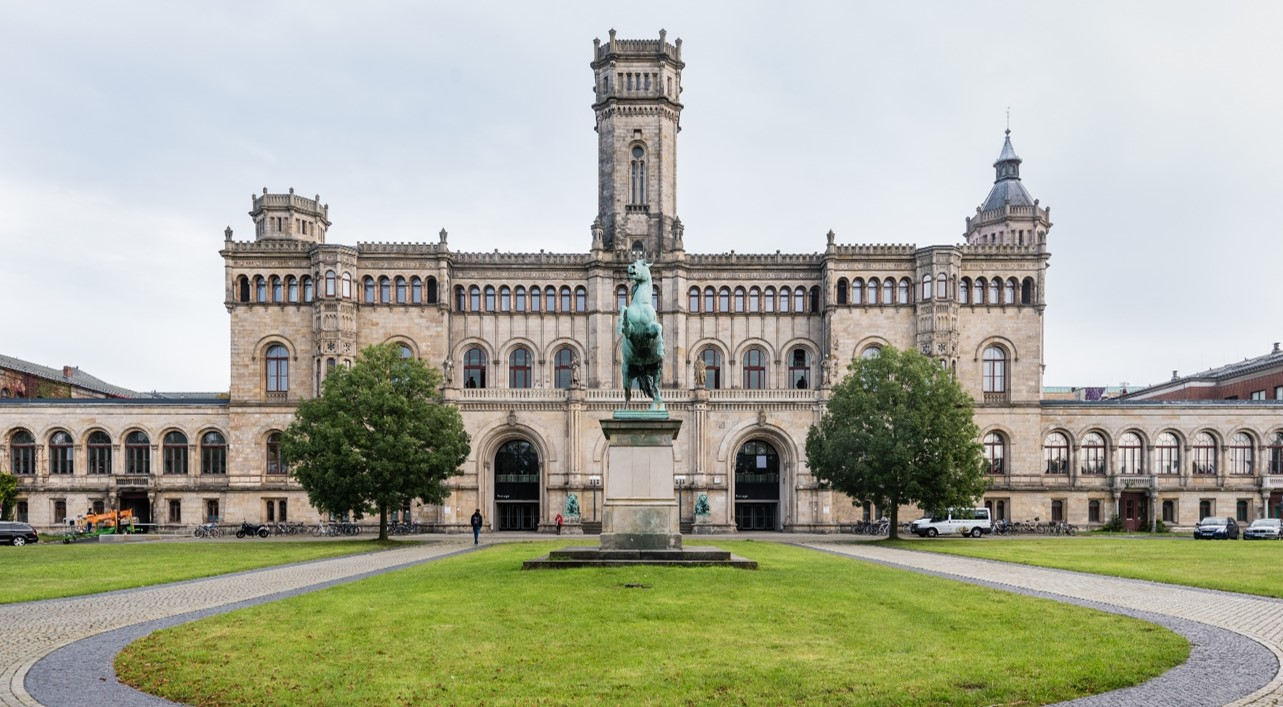
\includegraphics[width=0.75\textwidth]{figures/luh_default_presentation_title_image.jpg}}

\author[Lindauer \& Anand]{Marius Lindauer and Avishek Anand\\[1em]
	
\includegraphics[height=\logoheight]{../latex_main/figures/luh_logo_rgb_0_80_155.pdf}\qquad

\includegraphics[height=\logoheight]{../latex_main/figures/TNT_darkv4}\qquad

\includegraphics[height=\logoheight]{../latex_main/figures/L3S.jpg}	}
\date{Winter Term 2021
}


%%% Custom Packages
%----------------------------------------------------------------------
% Create dummy content
\usepackage{blindtext}

% Adds a frame with the current page layout. Just call \layout inside of a frame.
\usepackage{layout}


\title[Introduction]{iML: Shapley Values}
\subtitle{Introduction}

%\institute{}


\begin{document}
	
	\maketitle
	

\begin{frame}{Shapley Values}
  We can use Shapley values to explain individual predictions $\hat{f}(\xi)$ of a machine learning model $\hat{f}$:
\begin{itemize}
  \item Players $\hat{=}$ feature values of i-the observation $x_j^{(i)}, j \in \mathcal{P}$.
  \item Features cooperate to produce a prediction $\hat{f}(x^{(i)}_1, x^{(i)}_2, \ldots, x^{(i)}_p)$.
  \item The value function / payout of coalition $S$ for observation $x^{(i)}$ is
    $$v(S) =  \hat{f}_{S} (\xi_S) - \mathbb{E} (\hat{f}(\xi))$$ 
    where $\xi_S = \{x_j^{(i)}\}_{j \in S}$ and $\hat{f}_S: \mathcal{X}_S \mapsto \mathcal{Y}$.
\item The marginal prediction $\hat{f}_S$ is defined as $\hat{f}_{S}(x_S^{(i)}) := \int_{X_C} \hat{f}(x_S, X_C)d P_{X_C}$
\begin{itemize}
    \item Similar as in PDPs.
\end{itemize}

\item Subtraction of $\mathbb{E}(\hat{f}(x))$ to achieve $v(\emptyset) = 0$.
\item By using the marginal prediction, we have defined what it means for features to be \alert{missing} for the prediction: We remove it by integrating over its distribution.
\end{itemize}

\end{frame}

\begin{frame}{Shapley Values}

\begin{center}
\vspace{-0.3cm}
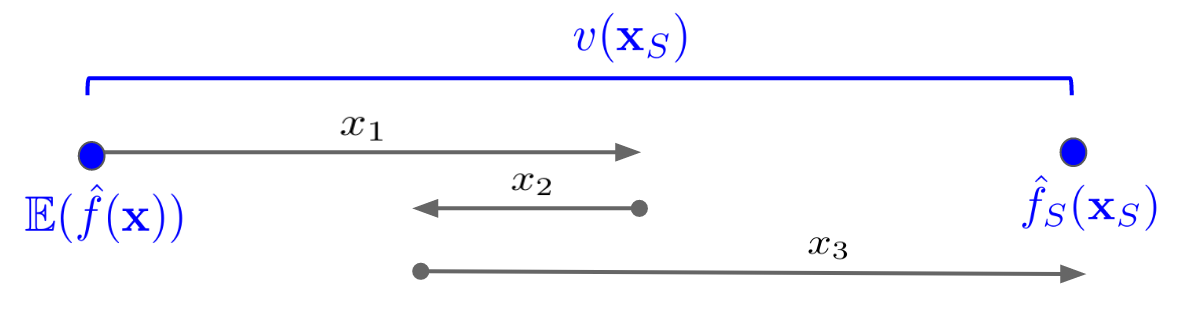
\includegraphics[width=0.8\textwidth]{figure/shapley_valuefct}
\end{center}

\begin{itemize}
     \item Shapley values tell us what the payout of each feature is
     \begin{itemize}
         \item how each feature contributes to the overall prediction of a specific observation.
     \end{itemize}
     \item The Shapley value is the average marginal contribution of a feature towards the prediction \textbf{across all possible feature coalitions}.
     \item The sum of Shapley values over all features yields the difference between the average prediction of all data points (baseline) and the selected individual prediction.
     \end{itemize}
\end{frame}

\begin{frame}{Shapley Value - Definition \lit{Strumbelj et al. 2014}{https://link.springer.com/article/10.1007/s10115-013-0679-x}}
  Using the order definition, the Shapley value for feature $j$ and a given data point $\xi$ can be computed as:
     $$ \phi^{(i)}_j  = \frac{1}{p!} \sum_{S \cup \{j\}} \underbrace{\hat{f}_{S \cup \{j\}}(x_{S \cup \{j\}}) - \hat{f}_{S}(x_{S})}_{\text{marginal contribution of feature $j$}} $$
\begin{itemize}
    \item The term $\mathbb{E}(\hat{f}(x))$ drops due to the subtraction of value functions.
  \item Interpretation of Shapley value $\phi^{(i)}_j$ for feature $j$ and observation $\xi$:
  The feature value $\xi_{j}$ contributed $\phi^{(i)}_j$ towards the prediction $\hat{f}(x)$ compared to the average prediction for the dataset.
   \item Note: Marginal contributions and Shapley values can be negative.
\end{itemize}
\tiny
\vfill
Shapley, Lloyd S. 1953. $"$A Value for N-Person Games.$"$\\
\end{frame}



\begin{frame}{Revisited: Axioms for Fair Attributions}
  We take the general axioms for Shapley Values and apply it to predictions:
  \begin{itemize}
    \item \textbf{Efficiency}: Feature contributions add up to the (centered) prediction. That means, unlike, e.g., LIME, we get a dense attribution, and not a sparse one.
      $\sum\nolimits_{j=1}^p\phi_j=\hat{f}(x)-E_X(\hat{f}(X))$
    \item \textbf{Symmetry}: Two feature that contribute the same to the prediction get the same payout. This ensures that, for example, interaction effects between two features are fairly divided. \\
      $\hat{f}_{S\cup\{j\}}(x_{\S \cup \{j\}}) = \hat{f}_{S \cup \{k\}}(x_{S \cup \{k\}})$ for all $S \subseteq P\setminus\{j,k\}$ then $\phi_j=\phi_k$
    \item \textbf{Dummy / Null Player}: The Shapley value of a feature that does not influence the prediction is zero. This means that if a feature was not selected by the model (e.g., tree or LASSO) the Shapley value is zero.  \\
      $\hat{f}_{S \cup \{j\}}(S \cup \{j\})=\hat{f}S(S)$ for all $S \subseteq P$ then $\phi_j=0$
    \item \textbf{Additivity}:  For a prediction with combined payouts, the
      payout is the sum of payouts: $\phi_j(v_1) + \phi_j(v_2)$. This means we can combine the Shapley values for model ensembles.
  \end{itemize}
\end{frame}



\begin{frame}{Estimation: A practical problem}
  \begin{itemize}
      \item Feature space is often high-dimensional.
      \item High-dimensionality is problematic for the (exact) Shapley value computation: For only 10 features, there are already $10! \approx 3.6$ million possible orders of features.
      \item We have a similar problem with the estimation of the marginal prediction: Averaging over the entire dataset for each (sampled) coalition would be very expensive.
      \item The solution to both problems is sampling. 
      \begin{itemize}
          \item Calculate Shapley value over $M$ samples. 
          \item For each sample, sample one order of features and one data point to replace missing features.
      \end{itemize}
      \item $M$ is a tradeoff between accuracy of the Shapley value and computational costs. 
      \begin{itemize}
          \item high $M$ $\leadsto$ better approximation of true Shapley values $\leadsto$ more costly computation
      \end{itemize}
  \end{itemize}
\end{frame}

\newcommand{\xk}{\mathbf{x}^{(k)}}

\begin{frame}{Estimation Algorithm}
Estimation for model $\hat{f}$, observation $\xi$, and sample size $M$:
  \begin{enumerate}
      \item For m in 1 to M, \textbf{do}:
      \begin{enumerate}
        \item Select random permutation $\pi \in \Pi$.
        \item Select random data point $x^{(k)} \in X$.
        \item Order $\xi$ according to $\pi$: $\xi_{\pi} = (x^{(i)}_{\pi(1)}, \ldots, x^{(i)}_{\pi(j)}, \ldots, x^{(i)}_{\pi(p)})$.
        \item Order $\xk$ according to $\pi$: $\xk_{\pi} = (x^{(k)}_{\pi(1)}, \ldots, x^{(k)}_{\pi(j)}, \ldots, x^{(k)}_{\pi(p)})$.
        \item Construct two instances:
          \begin{itemize}
            \item $\mathbf{x}_{+j} = (x^{(i)}_{\pi(1)}, \ldots, x^{(i)}_{\pi(j - 1)}, x^{(i)}_{\pi(j)}, x^{(k)}_{\pi(j + 1)}, \ldots, x^{(k)}_{\pi(p)}) $
            \item $\mathbf{x}_{-j} = (x^{(i)}_{\pi(1)}, \ldots, x^{(i)}_{\pi(j - 1)}, x^{(k)}_{\pi(j)}, x^{(k)}_{\pi(j + 1)}, \ldots, x^{(k)}_{\pi(p)}) $
          \end{itemize}
        \item Compute difference $\phi_j^m = \hat{f}(\mathbf{x}_{+j}) - \hat{f}(\mathbf{x}_{-j})$.
      \end{enumerate}
    \item Compute Shapley value $\phi_j = \frac{1}{M}\sum_{m=1}^M \phi_j^m$.
  \end{enumerate}

  Each $\phi_j^m$ is a sample from the marginal contribution for a sampled coalition.

  \tiny{Strumbelj, Erik, Igor Kononenko, Erik Strumbelj, and Igor Kononenko. 2014. $"$Explaining prediction models and individual predictions with feature contributions.$"$}

\end{frame}

\begin{frame}{Additional Estimation Trick}

  \vspace{-1em}
  The Shapley value can be estimated more efficiently when certain coalitions are always included in the computation, instead of relying on chance to sample them.
  \begin{itemize}
    \item The coalition with $S = \emptyset$ (i.e., $|S| = 0$) and $S = \{1, \ldots, p\} \setminus j$ have the highest weights in the Shapley value computation. By including them on purpose, the Shapley value becomes more stable with fewer samples. Sample weights have to be adapted for the sampled coalitions afterwards.
    \item Intuition: 
    \begin{itemize}
        \item Adding a feature to the empty coalition gives information about the \textit{pure} first order effect of the feature, which is the effect without any interactions.
        \item Adding the feature value to the otherwise complete set of feature values gives us the information about the total effect of a feature, which is the main effect affecting all interaction effects with other features.
    \end{itemize} 
    \item For coalition $S = \emptyset$, there are $0! (|P| - 0 - 1)! = 1 \cdot (|P| - 1)! = (p - 1)!$ orders, which is the same for $S = P \setminus \{j\}$: $|P \setminus \{j\}|! (|P| - |P \setminus \{j\}| - 1)! = (p - 1)! (p - (p-1) - 1)! = (p-1)!$.
    \end{itemize}
\end{frame}

\begin{frame}{Example: Additional Estimation Trick} 
    \begin{itemize}
    \item An example with $p = 5$ features:
      \begin{itemize}
        \item There are $5! = 120$ orders in total.
        \item In $(5 - 1)! = 24$ orders, we added feature value $x_j^{(i)}$ to the empty set.
        \item In 24 orders, we added the feature value to the otherwise full feature set.
        \item That means with just two sets, we can already get $\frac{48}{120} = 0.4$ of the contributions to the Shapley value.
      \end{itemize}
     \end{itemize}
\end{frame}

\begin{frame}{Example: Additional Estimation Trick (cont'd)} 
    
\begin{itemize}
    \item Similarly, we could proceed with all coalitions of $\{S: |S| = 1\}$ and $\{S: |S| = p - 1\}$.
    \item When some coalitions are added {manually}, and the rest are sampled, we have to adapt the weights: Let $w$ be the weight of the {manually} sampled coalitions, $\hat{\phi}_{j,fixed}$ the part of the Shapley value with only the manual contributions and $\hat{\phi}_{j,sample}$ the Shapley value with the sampled coalitions, then the Shapley value is: $w \cdot \hat{\phi}_{j,fixed} + (1 - w) \hat{\phi}_{j,sample}$.
  \end{itemize}

  \begin{center}
    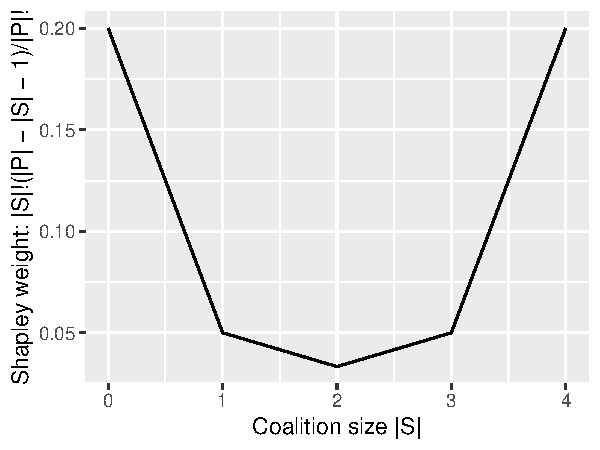
\includegraphics[width=0.35\textwidth]{figure/shapley-weights}
  \end{center}
\end{frame}

\begin{frame}{Bike Sharing Dataset}

\begin{center}
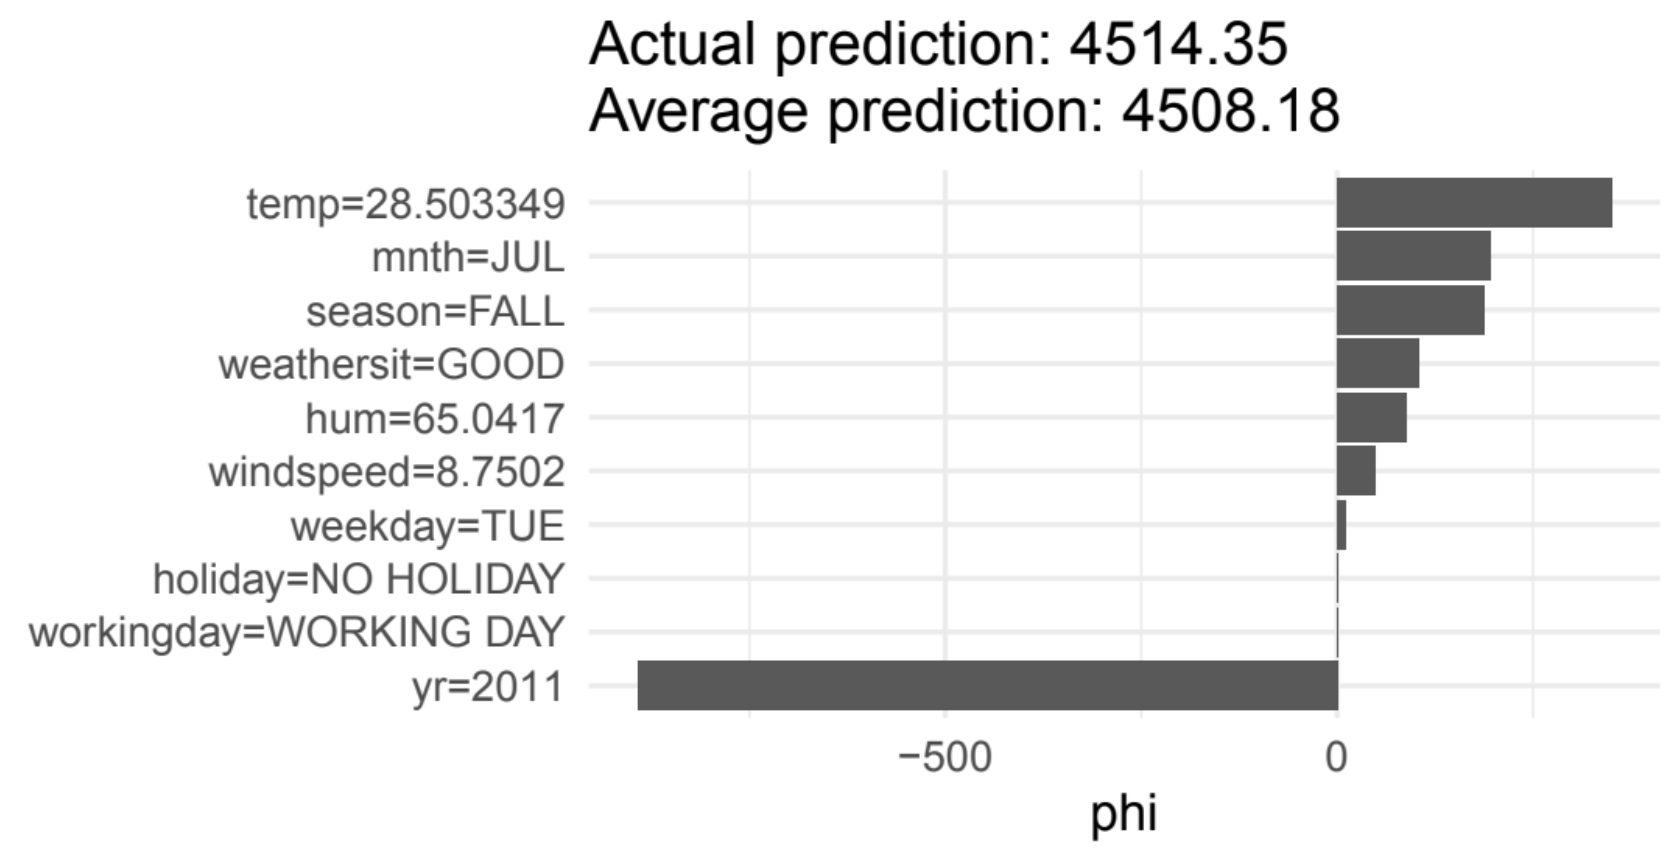
\includegraphics[width=0.85\textwidth]{figure/bike-sharing03.png}
\end{center}

The plot shows the Shapley values for observation 200.
The difference between the model prediction of this observation and the average prediction of the data is fairly distributed among the features (i.e., 4514 - 4508).
The most positive effect had feature value temp=28.5, with a contribution (increase of prediction) of + 350.
\end{frame}

\begin{frame}{Versions of the Shapley Value \lit{Lundberg et al. 2017}{https://arxiv.org/abs/1705.07874} \lit{Lundberg et al. 2018}{https://arxiv.org/abs/1802.03888}}

  \begin{itemize}
  \item KernelSHAP formulates the Shapley value solution as a regression problem using a specific kernel function. The authors show parallels to LIME and Deeplift.
  \item TreeSHAP is a fast Shapley value computation method for tree-based models such as gradient boosted trees.
 \end{itemize}
\end{frame}


\end{document}
